\section{Implementation}
\label{Implementation section}
As was stated in the introduction, we have two main implementations: 
\subsection{Simplistic Python implementation}
The Python implementation uses simplistic quadcopter dynamics only defined by:
\begin{itemize}
    \item Quad mass: $m_b$
    \item Moments of inertia: $I_{xx}$, $I_{yy}$, $I_{zz}$
    \item drag coefficient: $A_{x}$, $A_{y}$, $A_{z}$
    \item PD attitude gains: $K_{\phi_{p}}$, $K_{\phi_{d}}$, $K_{\psi_{p}}$, $K_{\psi_{d}}$, $K_{\theta_{p}}$, $K_{\theta_{d}}$. $\phi$ is the roll angle, $\theta$ is the pitch angle and $\psi$ is the yaw angle.
\end{itemize}

In this subsection, we will consider $q\in\mathbb{R}_6$ to be the rotational and translational states: $q(t) = (x(t), y(t), z(t), \phi(t), \theta(t), \psi(t))$
and $\dot{q}(t) = \frac{dq}{dt} = (\dot{x}(t), \dot{y}(t), \dot{z}(t), \dot{\phi}(t), \dot{\theta}(t), \dot{\psi}(t))$

It should be noted that the drag coefficients here are used both by the PVFC controller and the dynamics of our system. 
In opposition to the Gazebo implementation, the drag experienced by the quad in the python implementation is also defined by those drag coefficients.
When running in Gazebo, the IRIS model has a real world drag that we do not control.

We use ODEint to evolve the state $(q,\dot{q}, \ddot{q})$ of the system by doing to following on each time step: 
\begin{itemize}
    \item First we compute the current Mass Matrix $M$, Coriolis Matrix $C$, Control Matrix $B$, gravity Matrix $G$. Since the mass of the system is constant, the translational parts of $M$ and $G$ are constants.
    Therefore, the only changes we have to take into account are for $C$ and $B$.
    \item Then we pass to the PVFC controller those dynamics together with the desired velocity field and compute a desired thurst vector.
    \item Given a desired cartesian thrust vector $\tau_{desired} \in \mathbb{R}_3$, we can decompose it into euler coordinate $(\alpha, \tau_{\phi_{desired}}, \tau_{\theta_{desired}}, \tau_{\psi_{desired}})$. 
    \item The quad uses a simple attitude PD to compute the final thrust $\tau(t) = (\tau_{{\phi}}(t), \tau_{{\theta}}(t), \tau_{{\psi}}(t)) $ in euler coordinate :
    \begin{align}
        \tau_{{\phi}}(t) = I_{xx}(K_{\phi_{d}}(\dot{\phi}_{desired} - \dot{\phi}(t))+K_{\phi_{p}}(\phi_{desired} - \phi(t)))\\ \nonumber
        \tau_{{\theta}}(t) = I_{yy}(K_{\theta_{d}}(\dot{\theta}_{desired} - \dot{\theta}(t))+K_{\theta_{p}}(\theta_{desired} - \theta(t)))\\ \nonumber
        \tau_{{\psi}}(t) = I_{zz}(K_{\psi_{d}}(\dot{\psi}_{desired} - \dot{\psi}(t))+K_{\psi_{p}}(\psi_{desired} - \psi(t)))\\ \nonumber
    \end{align}
    \item By multiplying the final euler thrust by the control matrix, we can obtain the new state of the quadcopter
\end{itemize}
It is important to notice that the big difference between the python implementation and the ROS/Gazebo/PX4 that we will later detail is that we do not explicitly use a PD attitude gains in the latter. 
The PX4 firmware of the IRIS model has its own low level attitude controller.


The desired velocity fields are computed using Sympy (A Python library for symbolic ) for easy field and field gradient computation. Since most fields we used are derived from potential functions, we can easily obtain the field and field jacobian required by PVFC by symbolically differentiating their potentials or shaping functions.

\subsection{Full Sensor Placement pipeline in ROS/Gazebo/Pixhawk 4}
In this implementation, we are using a real world quadrotor called IRIS quad provided in the Pixhawk 4 SITL package. 
The dynamics are evolved and computed by Gazebo. 
The implementation is divided in 2 ROS Nodes, 1 ROS-PCL Node, 1 Gazebo-ROS plugin, and 1 Pixhawk 4/MAVROS node.
A diagram of the implementation is shown in figure \ref{fig:implementationdiagram}.
\subsubsection{Velocity Field ROS Node}
This node subscribes to the mavros odometry topic, computes the velocity field at the current position and publishes the desired field and field gradient. 
We implemented all the velocity field using the symbolic math library SymEngine so that all gradient computations from potential or shaping function would be done automatically. 
In addition, this node is implementing a state machine such that in each state, a specific field is being used.
Specifically, the first state gives a sink to get altitude, the second state is a sink field to approach the target, 
the third state represents the contact phase with the wall (the node subscribes to a topic called "grasping" to know if the grasping arm is currently activated). It starts when an engagement signal is received from the grasping arm and it finishes when a disengagment signal is received from the grasping arm. 
The last state is to get away from the wall and land, we use a sink field to implement it.
We implemented an obstacle avoidance system for generic superquadratic obstacles, upon obstacle detection, we compute the avoidance field for this obstacle from the appropriate shaping function, an irrotational field is generated to avoid the obstacle. This node subscribes to an obstacle topic to know when new obstacles have been detected. 
\subsubsection{PVFC ROS Node}
This node subscribes to the desired velocity field and to the MAVROS odometry and publishes a thurst vector on the MAVROS attitude topic computed by the PVFC controller. The output of the passive velocity field controller is a 4-dimensional vector containing the desired thrust to be applied in each direction $(x,y,z, fly)$ including the thurst to be applied on the fictitious flywheel. 
However, the input control for the IRIS model needs a desired attitude and thurst amplitude. Therefore, after obtaining the desired (cartesian) thrust vector from PVFC, we convert it to desired euler angles with desired amplitude $(\alpha, roll, pitch, yaw)$. 
We can then convert this pose to quaternion and publish it to the attitude topic of the IRIS quad.
It should be noted that the thrust amplitude expected by the IRIS attitude control is not in Newtons but is a scalar between 0 and 1. As a result, we had to experimentally calibrate a thrust slope and thrust intercept (affine transformation) to map the desired PVFC thurst amplitude to a scaled thurst amplitude. 
\subsubsection{PCL Object Segmentation Node}
This node reuses the code of a PCL tutorial performing cylinder segmentation on point cloud data(cite). 
We added a ROS integration to the velocity field topic the position of the detected object and also we implemented the transforms from camera point of view to FCU (Flying control unit) frame, and from FCU frame to world frame. 
It works in the following way:
\begin{itemize}
    \item Use a PCL passthrough filter to remove Nan datapoints and the scene background
    \item Use the PCL NormalEstimation class to estimate the normals of the cleaned pointcloud scene. This is done using KdTree based methods for increased robustness against noise in the measurements. KdTrees are data structures used in Computer Science that are very efficient for nearest neighbour search
    \item Perform plane model segmentation on the extracted normals using RANSAC and filter out the planar inliers
    \item After the last step, we should have a clean normals containing only cylinders normals, we can now use the SACSegmentationFromNormals class of PCL to extract the coefficient of the cylinder and its position in the frame of the camera
    \item If a cylinder was detected, we transform the position of the cylinder from the depth camera frame to the gazebo world frame and we publish it to the cylinder topic for the velocity field node to update the desired velocity field
\end{itemize}
\subsubsection{Grasping arm Gazebo-ROS plugin}    
This node reuses the code of the vaccuum arm of Gazebo, but it was modified so that could be "attached" to the moving IRIS model and fixed to a wall in Gazebo. 

\begin{figure*}[h!]
    \centering
    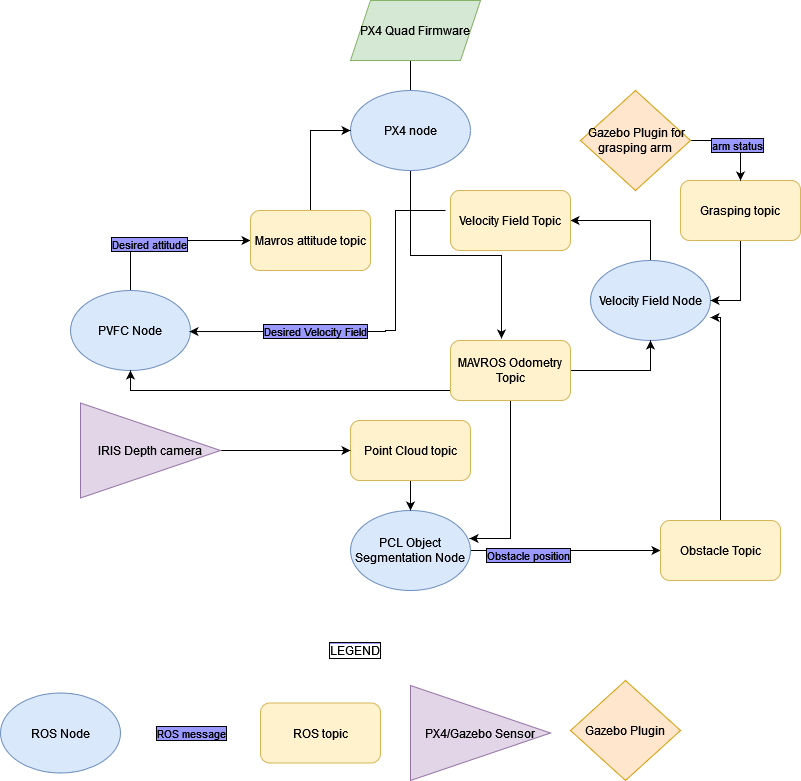
\includegraphics[width=\linewidth]{Images/implementation diagram.png}
    \caption{implementation diagram}
    \label{fig:implementationdiagram}
\end{figure*}
\newpage
